\begin{framed}

Objetivos:
\begin{itemize}
    \item Repasar el rol de la ecuación de estado en mecánica de fluidos.
    \item Repasar conceptos de termodinámica relevantes en flujos compresibles.
    \item Estudiar la propagación de ondas de presión en flujos compresibles.
\end{itemize}

Contenidos:
\begin{itemize}
    \item Ecuaciones de conservación en mecánica de fluidos para flujos incompresibles y compresibles. 
    \item La ecuación de estado para gases ideales. 
    \item Constantes termodinámicas.
    \item Energía interna, entalpía y entropía.
    \item Procesos isentrópicos.
    \item Ondas de presión
    \item El cono de Mach. 
\end{itemize}

Bibliografía:
\begin{itemize}
    \item Fox, R. W., Pritchard, P. J. y McDonald, A. T. (2009) Introduction to Fluid Mechanics. John Wiley \& Sons. Sección 9.6-9.7.
    \item White, F. M. (2008) Mecánica de Fluidos. McGraw-Hill. Sexta edición. Secciones 7.5-7.6.
\end{itemize}
\end{framed}

\section*{Ecuaciones de conservación y de estado en mecánica de fluidos}

Hasta ahora, hemos limitado nuestros análisis a flujos incompresibles.
A pesar de que ningún fluido es realmente incompresible (pues implicaría una velocidad del sonido infinita), para líquidos y gases a baja velocidad, esto es una buena aproximación.
En esta parte del curso vamos a tratar flujos compresibles, donde la variación de densidad juega un rol importante.
Una ventaja de los flujos incompresibles, es que hay ecuaciones que se esconden un poco de nosotros.
De hecho, estamos acostumbrados a tratar con la ecuación de continuidad y Navier-Stokes solamente:
%
\begin{align}\label{eq:incompresible}
\nabla\cdot\mathbf{V} &= 0\nonumber\\
\frac{D\mathbf{V}}{D t} &=-\frac{\nabla p}{\rho} +\nabla^2\mathbf{V}.
\end{align}
%
Sin embargo, también está la ecuación de conservación de la energía
%
\begin{equation}\label{eq:energia_incomp}
\rho c_p\frac{DT}{Dt} = -\nabla\cdot (\kappa\nabla T)
\end{equation}
%
donde $T$ es la temperatura, $c_p$ el calor específico a presión constante, y $\kappa$ el coeficiente de conductividad del medio.
La razón por la que comúnmente no operamos con la Ec. \eqref{eq:energia_incomp} es que para el caso incompresible no hay cambio de densidades debido a la temperatura, lo que desacopla la conservación de energía de la de momentum, y, a menos que queramos calcular el campo de temperaturas, no necesitamos la Ec. \eqref{eq:energia_incomp}.
Además, implícitamente hemos usado la ecuación de estado
%
\begin{equation}\label{eq:estado_incomp}
\rho = \text{constante}
\end{equation}
%
En general, necesitamos las cuatro o más ecuaciones para tener un sistema cerrado y modelar mecánica de fluidos, sin embargo, hasta ahora nos hemos focalizado en el caso fácil, donde necesitamos solamente dos de esas ecuaciones.

Volvamos un poco más atrás en las derivaciones para ver por qué necesitamos tantas ecuaciones.
En general, la ecuaciones de conservación de masa, momentum y energía son:
%
\begin{align}\label{eq:conservacion}
\frac{\partial\rho}{\partial t} + \nabla\cdot(\rho\mathbf{V})&=0\nonumber\\
\rho\frac{D\mathbf{V}}{Dt} &= -\nabla p + \nabla\cdot\tau_{ij}\nonumber\\
\rho\frac{D}{Dt}\left(u+\frac{p}{\rho}\right) &= \frac{Dp}{Dt}+\nabla\cdot(\kappa\nabla T) + \tau_{ij}\frac{\partial u_i}{\partial x_j}
\end{align}
%
donde $\tau_{ij}$ es el tensor con los esfuerzos de corte y $u$ la energía interna específica.
Si se fijan en la Ec. \eqref{eq:conservacion} tenemos 9 variables a calcular: $\rho$, $\mathbf{V}=(V_x,V_y,V_z)$, $p$, $\tau_{ij}$, $u$, $\kappa$ y $T$, sin embargo, solamente hay 5 ecuaciones (una de momentum por cada dirección, más energía y continuidad).
Para cerrar el sistema, necesitamos 4 ecuaciones más.
Una de estas ecuaciones las podemos sacar de relaciones constitutivas, o sea, ecuaciones propias del material. 
Por ejemplo, al asumir un fluido Newtoniano encontramos una relación entre la velocidad y $\tau_{ij}$ (de hecho, la usamos para llegar a la ecuación de Navier-Stokes).
El resto de las ecuaciones serán ecuaciones de estado, y las sacaremos de termodinámica.

\subsection*{Flujo no viscoso y ecuación de gas ideal}
Vamos al caso que nos interesa a nosotros.
En este curso, veremos flujos donde la compresibilidad es dominante frente a efectos viscosos, y asumiremos $\tau_{ij}=0$.
De esta forma, la Ec. \eqref{eq:conservacion} queda:
%
\begin{align}\label{eq:conservacion_novisc}
\frac{\partial\rho}{\partial t} + \nabla\cdot(\rho\mathbf{V})&=0\nonumber\\
\rho\frac{D\mathbf{V}}{Dt} &= -\nabla p \nonumber\\
\rho\frac{D}{Dt}\left(u+\frac{p}{\rho}\right) &= \frac{Dp}{Dt}+\nabla\cdot(\kappa\nabla T) 
\end{align}
%
donde la conservación de cantidad de movimiento nos llevó a la ecuación de Euler.
Para cerrar el sistema, necesitamos dos ecuaciones de estado, considerando que tenemos valores empíricos para $\kappa$.

Afortunadamente de termodinámica sabemos que con dos parámetros termodinámicos se define un estado, por lo tanto la energía interna es función de dos variables intependientes, por ejemplo $u=u(v_e,T)$, donde $v_e=1/\rho$ es el volúmen específico.
Por esto, podemos escribir
%
\begin{equation}\label{eq:denergia_interna}
du = \left(\frac{\partial u}{\partial T}\right)_vdT + \left(\frac{\partial u}{\partial v_e}\right)_Tdv_e
\end{equation}
%
Aquí aparece una definición que debiesen reconocer:
%
\begin{equation}
c_v = \left(\frac{\partial u}{\partial T}\right)_v
\end{equation}
%
que se conoce como el calor específico a volumen constante.
Quizás se acuerden en palabras: el calor específico es la cantidad de energía necesaria para subir un grado la temperatura.

Para la segunda ecuación de estado haremos una suposición: digamos que el fluido es un gas ideal, por lo tanto:
%
\begin{equation}\label{eq:gas_ideal}
\frac{p}{\rho} = RT
\end{equation}
%
donde $R=R_u/PM$ es la constante del gas, igual al ratio entre la constante  universal de gases sobre el peso molecular.
$R_u$ no es más que el ratio entre la constante de Boltzmann y el número de Avogadro.
No haremos la derivación al respecto, pero la ecuación de gases ideales (Ec. \eqref{eq:gas_ideal}) puede ser obtenida a partir de conceptos de mecánica estadística. 
Si consideramos las moléculas del gas como masas puntuales que no chocan entre ellas, al integrar sobre todas las posibles conformaciones de dichas moléculas, llegamos a la Ec. \eqref{eq:gas_ideal}.
Esto nos dice mucho de la validez del modelo: si consideramos que las moléculas no chocan entre ellas, significa que el gas tiene que estar muy diluído, con las moléculas muy separadas, y que la viscosidad no es importante.
Llega ser increíble que un modelo tan ``burdo'' funcione, pero la experiencia nos dice que en aire a $1$atm, la ecuación de gases ideales funciona muy bien para temperaturas sobre $-130^\circ$C (menos de 1\% de error).

Veamos un poco más de cerca el efecto de la suposición de gas ideal en la energía interna $u$.
La energía interna es la sumatoria de energía cinética (lineal y de rotación) y potencial (electrostática, van der Waals, etc.) de cada molécula de la sustancia, y para el caso ideal (sin colisiones) monoatómico, llegamos a que
%
\begin{equation}
u = \frac{3}{2}RT.
\end{equation}
%
Por lo tanto, en gases ideales la energía interna es solamente función de la temperatura.
Viendo la Ec. \eqref{eq:denergia_interna}, $\partial u/\partial v_e=0$, podemos reescribirla como:
%
\begin{equation}\label{eq:energia_interna}
du = c_vdT\Rightarrow u=c_vT,
\end{equation}
%
que es una relación que debiesen reconocer de sus clases de termodinámica.
De esta forma, quedamos con 7 variables en la Ec. \eqref{eq:conservacion_novisc} (sin considerar $\kappa$, que podemos obtener de tabla), y 7 ecuaciones (3 de momentum, continuidad, energía y 2 de estado), por lo que tenemos un sistema cerrado.

\subsection*{Otras variables termodinámicas}
\paragraph*{Entalpía}
Se hace conveniente definir otras variables que comúmente usamos en termodinámica.
Por ejemplo, la entalpía se define como:
%
\begin{equation}\label{eq:entalpia}
h = u+ pv_e,
\end{equation}
%
y, en general, depende de dos variables, por ejemplo $h=h(T,p)$.
Al derivar esta expresión, llegamos a lo siguiente:
%
\begin{equation}
dh = \left(\frac{\partial h}{\partial T}\right)_pdT + \left(\frac{\partial h}{\partial p}\right)_Tdp.
\end{equation}
%
Ahora, para el caso de gas ideal y usando la Ec. \eqref{eq:gas_ideal} podemos reescribir la Ec. \eqref{eq:entalpia} como
%
\begin{equation}
h = c_pT + RT
\end{equation}
%
lo que nos indica que, tal como $u$, $h$ depende de la temperatura solamente.
Esto nos lleva a decir que $\partial h/\partial p=0$ y
%
\begin{align}\label{eq:dentalpia}
dh &= \left(\frac{\partial h}{\partial T}\right)_pdT = c_pdT\nonumber\\
\Rightarrow h &= c_pT
\end{align}
%
donde $c_p$ es el calo específico a presión constante.

Comparemos las Ecs. \eqref{eq:denergia_interna} y \eqref{eq:dentalpia}.
Sabemos que para gases ideales
%
\begin{align}
h = u + RT &\Rightarrow dh = du + RdT\nonumber\\
&\Rightarrow dh = c_pdT = c_vdT + RdT\nonumber\\
&\Rightarrow c_p-c_v=R.
\end{align}
%
No deja de ser sorprendente que la resta entre dos variables que dependen de la temperatura de una constante, pero se da que su diferencia es constante.

También podemos definir el ratio de calores específicos:
%
\begin{equation}
k = \frac{c_p}{c_v}
\end{equation}
%
que para el caso de gases es $\sim1.4$.

\paragraph*{Entropía}
A partir de la segunda ley de la termodinámica, se puede deducir la desigualdad de Clausius
%
\begin{equation}\label{eq:clausius}
\oint \frac{dQ}{T}\leq0,
\end{equation}
% 
donde la igualdad en la indica un proceso reversible:
%
\begin{equation}\label{eq:clausius_rev}
\oint \frac{dQ}{T}=0
\end{equation}
%
y la desigualdad es válida para un proceso irreversible
%
\begin{equation}
\oint\frac{dQ}{T}<0.
\end{equation}

A partir de esto, se hace útil definir una nueva variable termodinámica, la entropía, como
%
\begin{equation}\label{eq:entropia}
dS = \left(\frac{dQ}{T}\right)_\text{reversible},
\end{equation}
%
Como nota al margen, la entropía tiene un significado muchísimo más profundo cuando la derivamos desde principios de mecánica estadística, pues guarda relación con la probabilidad de tener un determinado estado energético.
Si un estado energético (dado por cierta distribución espacial y energética de las moléculas) es más probable, su entropía será mayor.
Esto hace evidente (y fundamental) la segunda ley de la termodinámica, que dice que la entropía siempre va aumentando.
Un sistema naturalmente tenderá a estados energéticos más probables, y por tanto, de mayor entropía, reafirmando la segunda ley.
Esto lo dejo ahí para quien esté interesado, sin embargo, en el contexto del curso la definición dada por la Ec. \eqref{eq:entropia} es más que suficiente.

En el caso reversible, la Ec. \eqref{eq:clausius_rev} nos dice que la integral de línea de $dQ/T$ sobre una curva cerrada es cero, lo que matemáticamente nos indica que la integral no depende de la trayectoria, si no que solamente de sus puntos de inicio y fin.
Por esto, en cualquier proceso reversible (no necesariamente cerrado), se da que
%
\begin{equation}
\int_1^2\frac{dQ}{T} = \left(\frac{dQ}{T}\right)_2 -\left(\frac{dQ}{T}\right)_1 = S_2-S_1.
\end{equation}

Ahora, si el flujo es adiabático $dQ=0$, y las ecuaciones quedan
%
\begin{equation}
ds = 0 
\end{equation}
%
Esta última ecuación además nos indica que un proceso reversible y adiabático es también isentrópico.

La definición de entropía además de la primera ley de la termodinámica nos permiten escribir lo siguiente:
%
\begin{equation}
du = dq + dw \Rightarrow Tds = du+pdv_e
\end{equation}
%
donde $s$ es la entropía específica (por unidad de masa).
Para gases ideales queda como
%
\begin{align}
ds &= \frac{du}{T}+\frac{p}{T}dv_e = c_v\frac{dT}{T}+R\frac{dv_e}{v_e}\nonumber\\
s_2-s_1 &= c_v\ln\left(\frac{T_2}{T_1}\right) + R\ln\left(\frac{v_{e,2}}{v_{e,1}}\right) 
\end{align}
%
En el caso isentrópico, $s_2-s_1=0$, y podemos escribir
%
\begin{align}
&c_v\ln\left(\frac{T_2}{T_1}\right) + R\ln\left(\frac{v_{e,2}}{v_{e,1}}\right)=0 \nonumber\\
&\left(\frac{T_2}{T_1}\right)\left(\frac{v_{e,2}}{v_{e,1}}\right)^{R/c_v}=1\nonumber\\
&\Rightarrow T_2v_{e,2}^{k-1}=T_1v_{e,1}^{k-1}=Tv_{e}^{k-1}=\text{constante}
\end{align}
%
y usando la ecuación de gas ideal llegamos a
%
\begin{align}\label{eq:isentropico}
\frac{T^k}{p^{1-k}}=\text{constante}\nonumber\\
\frac{p}{\rho^k}=\text{constante}
\end{align}

\section*{Propagación de ondas de presión}

Una onda de presión (por ejemplo, de sonido), es la propagación por el medio de una perturbación en la presión.
Por ejemplo, si tenemos un receptáculo cerrado con aire, y lo golpeamos, localmente cerca de la pared la presión cambia, y este cambio en la presión viaja dentro del receptáculo.
Las ondas de presión se propagan a través del medio con una velocidad característica que llamaremos $c$, la velocidad del sonido, y a continuación la derivaremos a partir de variables termodinámicas.

Usemos la Figura \ref{fig:onda_presion} para guiar la discusión.
Digamos que el aire está quieto y de alguna forma perturbamos la presión un diferencial $dp$ en un lado, y la mantenemos.
Esto generará un frente de onda que viaja con velocidad $c$ en el eje $x$, donde en las zonas donde todavía no ha pasado el frente la velocidad seguirá siendo cero (aire quieto), la densidad será $\rho$ y la presión $p$.
Detrás del frente de onda, el cambio en presión a $p+dp$ genera movimiento del fluido con velocidad $dV_x$, y variación de densidad a $\rho+d\rho$.
%
\begin{figure}
\centering
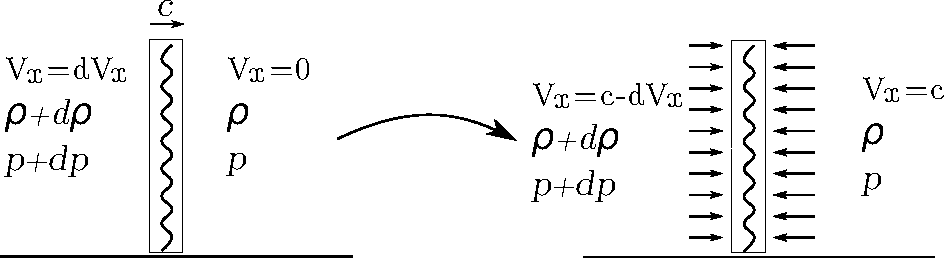
\includegraphics[width=0.8\textwidth]{clase13/onda_presion.pdf}
\caption{Análisis de volumen de control sobre una onda de presión. La figura a la izquierda usa un volumen de control en movimiento, y la de la derecha considera un observador que se mueve con el volumen de control.}
\label{fig:onda_presion}
\end{figure}

Analicemos el sistema como un observador que se mueve con la onda de presión.
Si hacemos un volumen de control que se mueve con la onda, nuestro observador verá como el flujo se entra al volumen de control con velocidad $c$, y sale de este con velocidad $c-dV_x$.
En el contexto de volúmen de control, la ecuación de continuidad es:
%
\begin{equation}
0 = \int_{VC}\rho d\vol + \oint_{SC}\rho \mathbf{V}\cdot\hat{n}dA
\end{equation}
%
donde la acumulación será cero (pues estamos en estado estacionario), y los flujos de entrada y salida tienen un perfil de velocidad constante.
Despreciando los términos con más de un diferencial (en otras palabras, linealizando), esto nos deja con:
%
\begin{align}\label{eq:continuidad_onda}
&-\rho c A + (\rho+d\rho)(c-dV_x)A = 0\nonumber\\
&\Rightarrow dV_x = \frac{c}{\rho}d\rho
\end{align}

Fijémonos ahora en la ecuación de momentum. 
Con análisis de volumen de control, esta ecuación es
%
\begin{equation}
\sum \mathbf{F} = \int_{VC}\mathbf{V}\rho d\vol + \oint_{SC}\mathbf{V}\rho \mathbf{V}\cdot\hat{n}dA
\end{equation}
%
donde la única fuerza es debido al cambio de presión ($F=dpA$), si no consideramos la gravedad.
Poniendo los valores de velocidad de entrada y salida del volumen de control, y usando la ecuación de continuidad, quedamos con
%
\begin{align}\label{eq:momentum_onda}
-dpA &= -\rho c^2A + (c-dV_x)^2(\rho+d\rho)A\nonumber\\
-dpA &= -\rho c^2A + (c-dV_x)\rho cA = (-c+c-dV_x)\rho cA\nonumber\\
\Rightarrow dV_x &= \frac{dp}{\rho c}
\end{align}
%
e igualando a la Ec. \eqref{eq:continuidad_onda} quedamos con
%
\begin{align}\label{eq:vel_sonido}
\frac{c}{\rho}d\rho = \frac{dp}{\rho c}\nonumber\\
\Rightarrow c^2 = \frac{dp}{d\rho}
\end{align}
%
lo que define la velocidad del sonido en cualquier medio a partir de termodinámica.

Fíjense en la implicancia física de la Ec. \eqref{eq:vel_sonido} en el caso incompresible.
Para flujos incompresibles, $d\rho=0$, por lo que la velocidad del sonido sería infinita!
En otras palabras, cualquier perturbación en un fluido incompresible sería ``sentido'' en todo el resto del dominio instantáneamente.

La variación de presión es infinitesimal, por lo tanto, puede considerarse como un proceso reversible, y además es rápido, por lo que no entrega tiempo para la liberación de calor, haciéndolo adiabático.
Por esto, pordemos decir que la onda de sonido es isentrópica (entropía constante):
%
\begin{align}\label{eq:vel_sonido}
\Rightarrow c^2 = \left.\frac{dp}{d\rho}\right|_{s=\text{constante}}
\end{align}
%
De hecho, puede ser más fácil darse cuenta del carácter isentrópico de una onda de presión pensando en términos de mećanica estadística.
La entropía es la probabilidad de tener un cierto estado energético (moléculas en cierto lugar con cierta energía cinética y potencial), y una pequeña onda de presión no tendrá un efecto notorio en las moléculas (seguirán igual de ``desordenadas'' y con una energía parecida), por lo que el estado energético no varía.

Ya vimos en la Ec. \eqref{eq:isentropico} que $p/\rho^k=$constante.
Diferenciemos esa expresión, y apliquemos el caso de gas ideal:
%
\begin{align}
&\frac{p}{\rho^k}=C\Rightarrow p = C\rho^k\nonumber\\
&\left.\ln(p) = \ln(C)+k\ln(\rho)\right/d\nonumber\\
&d(\ln(p)) =d(\ln(C)) + kd(\ln(\rho))\nonumber\\
&\frac{dp}{p} = k\frac{d\rho}{\rho}\nonumber\\
&\Rightarrow \frac{dp}{d\rho} = k\frac{p}{\rho} = kRT.
\end{align}
%
Por lo tanto, podemos escribir la velocidad del sonido en un flujo ideal como 
%
\begin{equation}
c=\sqrt{kRT}
\end{equation}

\subsection*{El cono de Mach}

A continuación, veremos qué ocurre si la fuente de la onda de presión es móvil, y se mueve con velocidad subsónica, sónica y supersónica.
Veamos cada caso, cuando la fuente emite tres ondas, $\Delta t_1$, $\Delta t_2$ y $\Delta t_3$ segundos antes del tiempo actual, y se mueve de derecha a izquierda.  

\begin{itemize}
\item $\mathbf{V=0}$: Este es el caso más simple, donde el fuente está quieta, y siempre al centro del frente esférico de las ondas de presión. 
La Figura \ref{fig:V0} es un ejemplo de esto
%
\begin{figure}[h!]
\centering
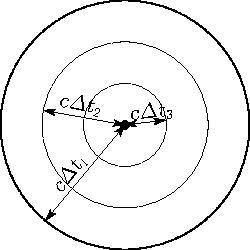
\includegraphics[width=0.4\textwidth]{clase13/V0.pdf}
\caption{Ondas de presión de una fuente quieta.}
\label{fig:V0}
\end{figure}
%
\item $\mathbf{V<c}$: la fuente viaja a velocidad subsónica, por lo que el frente de la onda de presión siempre va adelante de la fuente.
La Figura \ref{fig:Vsub} es un ejemplo de esto
%
\begin{figure}[h!]
\centering
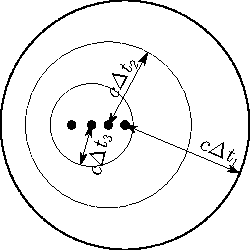
\includegraphics[width=0.4\textwidth]{clase13/Vsub.pdf}
\caption{Ondas de presión de una fuente que se mueve con velocidad subsónica.}
\label{fig:Vsub}
\end{figure}
%
\item $\mathbf{V=c}$: la fuente viaja a la velocidad del sonido, por lo que se encuentra sobre el frente de onda.
Debido a esto, la amplitud de la onda crece donde se encuentra la fuente, aumentando localmente la presión.
Es este aumento de presión el responsable de que sea tan difícil pasar la barrera del sonido (de ahí el nombre ``barrera'').
La Figura \ref{fig:Vsonico} es un ejemplo de esto
%
\begin{figure}[h!]
\centering
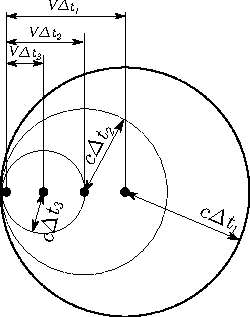
\includegraphics[width=0.4\textwidth]{clase13/Vsonico.pdf}
\caption{Ondas de presión de una fuente que se mueve con la velocidad del sonido.} 
\label{fig:Vsonico}
\end{figure}
%
\item $\mathbf{V>c}$: la fuente viaja a velocidad supersónica, por lo que se encuentra adelante del frente de onda.
Como vemos a partir de la Figura \ref{fig:Vsuper}, se genera una onda oblicua (cónica en tres dimensiones) donde fuera del cono la onda todavía no llega.
Este cono se conoce como el \emph{cono de Mach}.
La Figura \ref{fig:Vsuper} nos muestra que se generan triángulos rectángulos, y se hace patente que el semiángulo del cono es:
%
\begin{equation}
\sin (\alpha) = \frac{c\Delta t}{V\Delta t} = \frac{c}{V}.
\end{equation}
%
En el contexto de flujo compresible, se hace más fácil adimensionalizar la velocidad con $c$, dando paso al número de Mach:
%
\begin{equation}
M = \frac{V}{c},
\end{equation}
%
y podemos reescribir el seno del semiángulo como
%
\begin{equation}
\sin(\alpha)= \frac{1}{M}
\end{equation}
%
\begin{figure}[h!]
\centering
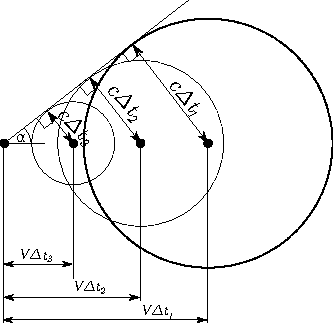
\includegraphics[width=0.6\textwidth]{clase13/Vsuper.pdf}
\caption{Ondas de presión de una fuente que se mueve con velocidad supersónica.} 
\label{fig:Vsuper}
\end{figure}
\end{itemize}


